\section{Occupancy Grid Map (OGM)}
\label{section:ogm}

Η αναπαράσταση του χώρου μετά από την εφαρμογή του αλγορίθμου SLAM\footnote{\href{http://wiki.ros.org/gmapping}{http://wiki.ros.org/gmapping}} πραγματοποιείται με την χρήση \emph{χαρτών πλέγματος κατάληψης} (Occupancy Grid Maps) στους διδιάστατους χώρους, όπως περιγράφεται από τους Wolf και Sukhatme \cite{ogm2005}. Αναπαρτιστά τον χώρο ως ένα σύνολο τετραγωνικών κελιών, στα οποία αποθηκεύεται πιθανότητα η κατάληψης τους. Το κάθε κελί μπορεί να πάρει τρεις διαφορετικές καταστάσεις που αντιστοιχούν στις παρακάτω τιμές:
\begin{itemize}
    \setlength\itemsep{-0.2em}
    \item 100 όταν είναι κατειλημμένο (obstacle).
    \item 0 όταν είναι ελεύθερο (free space).
    \item -1 όταν είναι άγνωστο το περιεχώμενο του σημείου (unknown).
\end{itemize}
Κατά τη διαδικασία του SLAM διαβάζονται οι μετρήσεις του αισθητήρα που χρησιμοποιείται και όσο αυτός δείχνει ότι μια θέση είναι ελεύθερη τόσο η τιμή του κελιού της στο OGM θα μειώνεται έως και την τιμή 0, ενώ αντίστοιχα όσο θα δείχνει ότι μια θέση είναι κατειλημμένη, τόσο η τιμή στο κελί του OGM θα αυξάνεται μέχρι την τιμή 100. Με αυτόν τον τρόπο ορίζεται η πιθανότητα κατάληψης των κελιών.

Στο \autoref{fig:sparse_3_ogm} παρουσιάζεται ένα OGM ενός χώρου που προέκυψε μετά από προσομοίωση SLAM στο Gazebo. Τα εμπόδια έχουν μαύρο χρώμα, ο ελεύθερος χώρος άσπρο και ο άγνωστος γκρι.
\begin{figure}
    \centering
    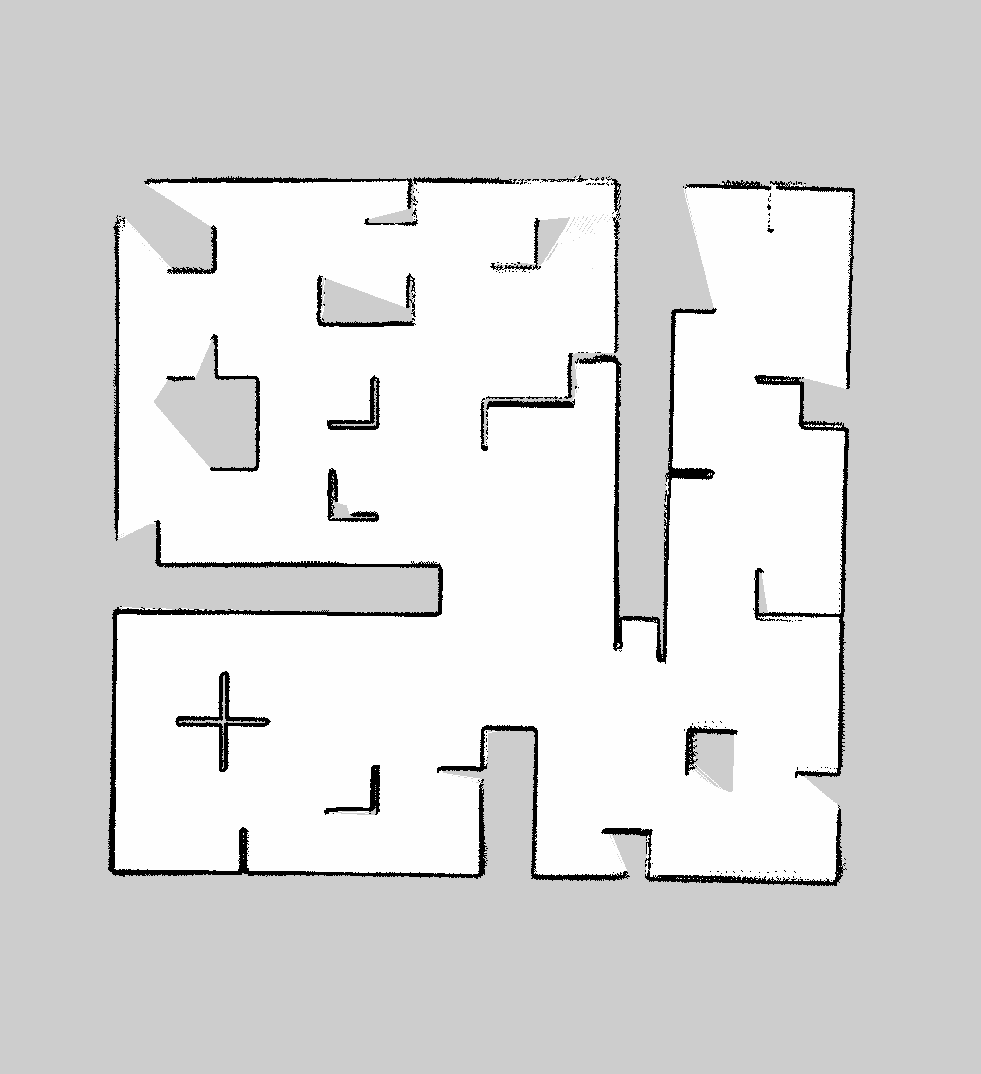
\includegraphics[width=0.5\textwidth]{./images/chapter3/sparse_3.png}
    \caption{Παράδειγμα ΟGM εικονικού χώρου}
    \label{fig:sparse_3_ogm}
\end{figure}




